\documentclass[tikz,border=5mm]{standalone}
\usepackage{tikz}
\usetikzlibrary{arrows.meta, positioning, calc}

% --- COLOR DEFINITIONS ---
\definecolor{Garnet}{HTML}{73000A}
\definecolor{CBlue}{HTML}{466A9F}
\definecolor{CGrayDark}{HTML}{333333} 
\definecolor{CGrayLight}{HTML}{E5E5E5}

\begin{document}
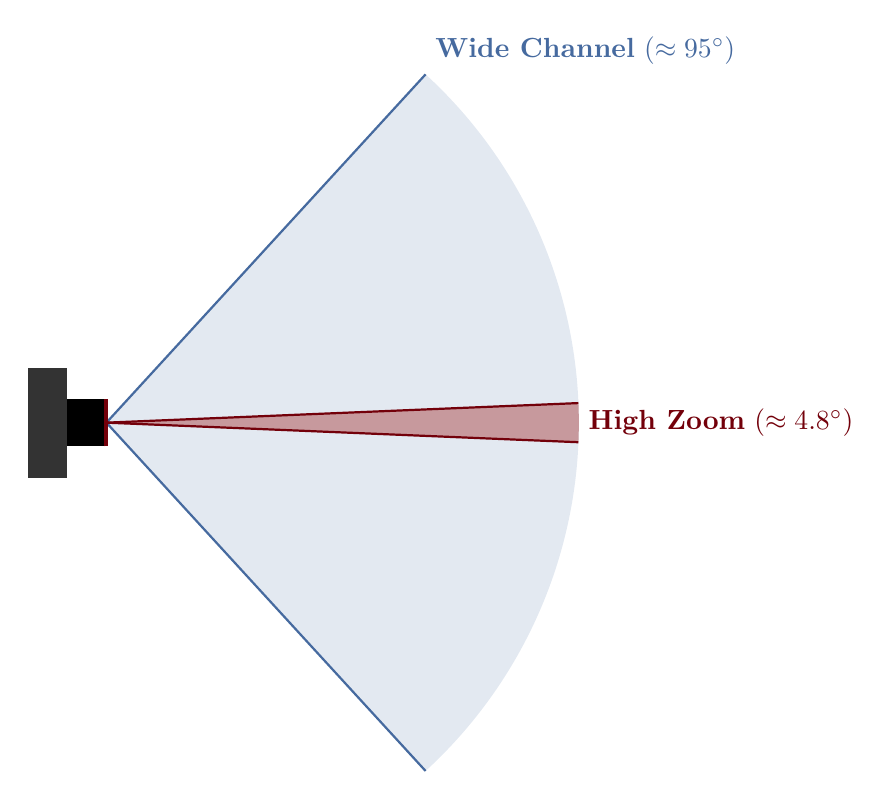
\begin{tikzpicture}
  % --- GEOMETRIC VARIABLES ---
  \def\Radius{6}
  \def\WideAngle{95}
  \def\WideHalf{\WideAngle/2}
  \def\ZoomAngle{4.75}
  \def\ZoomHalf{\ZoomAngle/2}
  
  % =====================================================================
  % 1. WIDE ANGLE (Background Layer)
  % =====================================================================
  % Fill
  \fill[CBlue!15] (0,0) -- (\WideHalf:\Radius) arc (\WideHalf:-\WideHalf:\Radius) -- cycle;
  % Border Lines
  \draw[CBlue, thick] (0,0) -- (\WideHalf:\Radius);
  \draw[CBlue, thick] (0,0) -- (-\WideHalf:\Radius);
  
  % Label for Wide
  % Placed along the top edge of the wide cone
  \node[CBlue, anchor=south west] at (\WideHalf:\Radius) {
    \textbf{Wide Channel} ($\approx 95^\circ$)
  };

  % =====================================================================
  % 2. HIGH ZOOM (Foreground Overlay)
  % =====================================================================
  % Fill (Opacity ensures it stands out against the blue)
  \fill[Garnet!40] (0,0) -- (\ZoomHalf:\Radius) arc (\ZoomHalf:-\ZoomHalf:\Radius) -- cycle;
  % Border Lines
  \draw[Garnet, thick] (0,0) -- (\ZoomHalf:\Radius);
  \draw[Garnet, thick] (0,0) -- (-\ZoomHalf:\Radius);
  
  % Label for Zoom
  % Placed at the very end (center)
  \node[Garnet, anchor=west] at (\Radius, 0) {
    \textbf{High Zoom} ($\approx 4.8^\circ$)
  };

  % =====================================================================
  % 3. CAMERA BODY (Shared Origin)
  % =====================================================================
  % Lens Housing
  \fill[black] (-0.5, -0.3) rectangle (0, 0.3);
  % Main Body
  \fill[CGrayDark] (-1, -0.7) rectangle (-0.5, 0.7);
  % Front Element Indicator
  \draw[Garnet, line width=1.5pt] (0, -0.3) -- (0, 0.3);

\end{tikzpicture}
\end{document}